% Created 2021-12-09 to 17:32
% Intended LaTeX compiler: pdflatex
\documentclass[12pt]{article}

%%%% settings when exporting code %%%% 

\usepackage{listings}
\lstdefinestyle{code-small}{
backgroundcolor=\color{white}, % background color for the code block
basicstyle=\ttfamily\small, % font used to display the code
commentstyle=\color[rgb]{0.5,0,0.5}, % color used to display comments in the code
keywordstyle=\color{black}, % color used to highlight certain words in the code
numberstyle=\ttfamily\tiny\color{gray}, % color used to display the line numbers
rulecolor=\color{black}, % color of the frame
stringstyle=\color[rgb]{0,.5,0},  % color used to display strings in the code
breakatwhitespace=false, % sets if automatic breaks should only happen at whitespace
breaklines=true, % sets automatic line breaking
columns=fullflexible,
frame=single, % adds a frame around the code (non,leftline,topline,bottomline,lines,single,shadowbox)
keepspaces=true, % % keeps spaces in text, useful for keeping indentation of code
literate={~}{$\sim$}{1}, % symbol properly display via latex
numbers=none, % where to put the line-numbers; possible values are (none, left, right)
numbersep=10pt, % how far the line-numbers are from the code
showspaces=false,
showstringspaces=false,
stepnumber=1, % the step between two line-numbers. If it's 1, each line will be numbered
tabsize=1,
xleftmargin=0cm,
emph={anova,apply,class,coef,colnames,colNames,colSums,dim,dcast,for,ggplot,head,if,ifelse,is.na,lapply,list.files,library,logLik,melt,plot,require,rowSums,sapply,setcolorder,setkey,str,summary,tapply},
aboveskip = \medskipamount, % define the space above displayed listings.
belowskip = \medskipamount, % define the space above displayed listings.
lineskip = 0pt} % specifies additional space between lines in listings
\lstset{style=code-small}
%%%% packages %%%%%

\usepackage[utf8]{inputenc}
\usepackage[T1]{fontenc}
\usepackage{lmodern}
\usepackage{textcomp}
\usepackage{color}
\usepackage{graphicx}
\usepackage{grffile}
\usepackage{wrapfig}
\usepackage{rotating}
\usepackage{longtable}
\usepackage{multirow}
\usepackage{multicol}
\usepackage{changes}
\usepackage{pdflscape}
\usepackage{geometry}
\usepackage[normalem]{ulem}
\usepackage{amssymb}
\usepackage{amsmath}
\usepackage{amsfonts}
\usepackage{dsfont}
\usepackage{array}
\usepackage{ifthen}
\usepackage{hyperref}
\usepackage{natbib}
%
%%%% specifications %%%%
%
\usepackage{ifthen}
\usepackage{xifthen}
\usepackage{xargs}
\usepackage{xspace}
\newcommand\Rlogo{\textbf{\textsf{R}}\xspace} %
\RequirePackage{fancyvrb}
\DefineVerbatimEnvironment{verbatim}{Verbatim}{fontsize=\small,formatcom = {\color[rgb]{0.5,0,0}}}
\RequirePackage{colortbl} % arrayrulecolor to mix colors
\RequirePackage{setspace} % to modify the space between lines - incompatible with footnote in beamer
\renewcommand{\baselinestretch}{1.1}
\geometry{top=1cm}
\RequirePackage{colortbl} % arrayrulecolor to mix colors
\RequirePackage{pifont}
\RequirePackage{relsize}
\newcommand{\Cross}{{\raisebox{-0.5ex}%
{\relsize{1.5}\ding{56}}}\hspace{1pt} }
\newcommand{\Valid}{{\raisebox{-0.5ex}%
{\relsize{1.5}\ding{52}}}\hspace{1pt} }
\newcommand{\CrossR}{ \textcolor{red}{\Cross} }
\newcommand{\ValidV}{ \textcolor{green}{\Valid} }
\usepackage{stackengine}
\usepackage{scalerel}
\newcommand\Warning[1][3ex]{%
\renewcommand\stacktype{L}%
\scaleto{\stackon[1.3pt]{\color{red}$\triangle$}{\tiny\bfseries !}}{#1}%
\xspace
}
\hypersetup{
citecolor=[rgb]{0,0.5,0},
urlcolor=[rgb]{0,0,0.5},
linkcolor=[rgb]{0,0,0.5},
}
\RequirePackage{epstopdf} % to be able to convert .eps to .pdf image files
\RequirePackage{capt-of} %
\RequirePackage{caption} % newlines in graphics
\RequirePackage{enumitem} % to be able to convert .eps to .pdf image files
\RequirePackage{amsmath}
\RequirePackage{algorithm}
\RequirePackage[noend]{algpseudocode}
\RequirePackage{dsfont}
\RequirePackage{amsmath,stmaryrd,graphicx}
\RequirePackage{prodint} % product integral symbol (\PRODI)
\newcommand\defOperator[7]{%
\ifthenelse{\isempty{#2}}{
\ifthenelse{\isempty{#1}}{#7{#3}#4}{#7{#3}#4 \left#5 #1 \right#6}
}{
\ifthenelse{\isempty{#1}}{#7{#3}#4_{#2}}{#7{#3}#4_{#1}\left#5 #2 \right#6}
}
}
\newcommand\defUOperator[5]{%
\ifthenelse{\isempty{#1}}{
#5\left#3 #2 \right#4
}{
\ifthenelse{\isempty{#2}}{\underset{#1}{\operatornamewithlimits{#5}}}{
\underset{#1}{\operatornamewithlimits{#5}}\left#3 #2 \right#4}
}
}
\newcommand{\defBoldVar}[2]{
\ifthenelse{\equal{#2}{T}}{\boldsymbol{#1}}{\mathbf{#1}}
}
\newcommandx\Cov[2][1=,2=]{\defOperator{#1}{#2}{C}{ov}{\lbrack}{\rbrack}{\mathbb}}
\newcommandx\Esp[2][1=,2=]{\defOperator{#1}{#2}{E}{}{\lbrack}{\rbrack}{\mathbb}}
\newcommandx\Prob[2][1=,2=]{\defOperator{#1}{#2}{P}{}{\lbrack}{\rbrack}{\mathbb}}
\newcommandx\Qrob[2][1=,2=]{\defOperator{#1}{#2}{Q}{}{\lbrack}{\rbrack}{\mathbb}}
\newcommandx\Var[2][1=,2=]{\defOperator{#1}{#2}{V}{ar}{\lbrack}{\rbrack}{\mathbb}}
\newcommandx\Binom[2][1=,2=]{\defOperator{#1}{#2}{B}{}{(}{)}{\mathcal}}
\newcommandx\Gaus[2][1=,2=]{\defOperator{#1}{#2}{N}{}{(}{)}{\mathcal}}
\newcommandx\Wishart[2][1=,2=]{\defOperator{#1}{#2}{W}{ishart}{(}{)}{\mathcal}}
\newcommandx\Likelihood[2][1=,2=]{\defOperator{#1}{#2}{L}{}{(}{)}{\mathcal}}
\newcommandx\Information[2][1=,2=]{\defOperator{#1}{#2}{I}{}{(}{)}{\mathcal}}
\newcommandx\Score[2][1=,2=]{\defOperator{#1}{#2}{S}{}{(}{)}{\mathcal}}
\newcommandx\Vois[2][1=,2=]{\defOperator{#1}{#2}{V}{}{(}{)}{\mathcal}}
\newcommandx\IF[2][1=,2=]{\defOperator{#1}{#2}{IF}{}{(}{)}{\mathcal}}
\newcommandx\Ind[1][1=]{\defOperator{}{#1}{1}{}{(}{)}{\mathds}}
\newcommandx\Max[2][1=,2=]{\defUOperator{#1}{#2}{(}{)}{min}}
\newcommandx\Min[2][1=,2=]{\defUOperator{#1}{#2}{(}{)}{max}}
\newcommandx\argMax[2][1=,2=]{\defUOperator{#1}{#2}{(}{)}{argmax}}
\newcommandx\argMin[2][1=,2=]{\defUOperator{#1}{#2}{(}{)}{argmin}}
\newcommandx\cvD[2][1=D,2=n \rightarrow \infty]{\xrightarrow[#2]{#1}}
\newcommandx\Hypothesis[2][1=,2=]{
\ifthenelse{\isempty{#1}}{
\mathcal{H}
}{
\ifthenelse{\isempty{#2}}{
\mathcal{H}_{#1}
}{
\mathcal{H}^{(#2)}_{#1}
}
}
}
\newcommandx\dpartial[4][1=,2=,3=,4=\partial]{
\ifthenelse{\isempty{#3}}{
\frac{#4 #1}{#4 #2}
}{
\left.\frac{#4 #1}{#4 #2}\right\rvert_{#3}
}
}
\newcommandx\dTpartial[3][1=,2=,3=]{\dpartial[#1][#2][#3][d]}
\newcommandx\ddpartial[3][1=,2=,3=]{
\ifthenelse{\isempty{#3}}{
\frac{\partial^{2} #1}{\partial #2^2}
}{
\frac{\partial^2 #1}{\partial #2\partial #3}
}
}
\newcommand\Real{\mathbb{R}}
\newcommand\Rational{\mathbb{Q}}
\newcommand\Natural{\mathbb{N}}
\newcommand\trans[1]{{#1}^\intercal}%\newcommand\trans[1]{{\vphantom{#1}}^\top{#1}}
\newcommand{\independent}{\mathrel{\text{\scalebox{1.5}{$\perp\mkern-10mu\perp$}}}}
\newcommand\half{\frac{1}{2}}
\newcommand\normMax[1]{\left|\left|#1\right|\right|_{max}}
\newcommand\normTwo[1]{\left|\left|#1\right|\right|_{2}}
\author{Brice Ozenne, Vibeke Dam}
\date{\today}
\title{Leveraging multimodal data to predict outcomes of antidepressant treatment\\\medskip
\large Preliminary results}
\hypersetup{
 colorlinks=true,
 pdfauthor={Brice Ozenne, Vibeke Dam},
 pdftitle={Leveraging multimodal data to predict outcomes of antidepressant treatment},
 pdfkeywords={},
 pdfsubject={},
 pdfcreator={Emacs 27.2 (Org mode 9.4.4)},
 pdflang={English}
 }
\begin{document}

\maketitle

\section{Data}
\label{sec:orga85803e}

The data (n=98) we use has been provided by Emily Beaman. She processed
relevant data from the CIMBI database. In addition we compute:
\begin{itemize}
\item a "MR" biomarker as the average of the thickness of the left
lateral, right lateral, left medial, and right medial orbitol
frontal cortex.
\item a "PET" biomarker by combining the log binding potential from
neocortex, hippocampus, caudate, and putamen via a latent variable
model (adjusted for age, gender, and injected mass). This was done
in a leave-one-out fashion i.e. the biomarker for individual \(i\)
was obtained by fitting the model on all but the i-th individual and
estimating the latent variable for the \(i\)-th individual based on
its log-binding in the 4 regions.
\item a "cognition" biomarker was obtained via a k-means algorithm on
various cognitive outcomes (no leave-one-out here).
\item the "outcomes" by computing the relative change in HAMD6 between week 8 (or 12) and baseline.
\end{itemize}
Individuals who had missing HAMD6 at both week 8 and 12 were excluded (n=13)

\bigskip

The corresponding R code is in the file \texttt{0-data-management.R} available on \href{https://github.com/bozenne/article-predictionNP1BD3/code-data-analysis}{Github}.

\clearpage

\section{Data analysis}
\label{sec:org5175886}

After discussion with neuroscientist, we have identified 10 candidate
biomarkers\footnote{fMRI is missing in the list} for predicting recovery after SSRI treatment:
\begin{itemize}
\item \texttt{MR\_OFCthick}: thickness of the OFC brain region measured with MR.
\item \texttt{HAMD17}: depression score at baseline.
\item \texttt{low\_hsCRP}: high sensitivity CRP (l levels of inflammation in the body).
\item \texttt{lvpet}: summary of the brain log-PET binding.
\item \texttt{cognitive\_cluster}: summary of the cognition
\item \texttt{EEG\_vigilance}: EEG signal (vigilance slope B1 bl)
\item \texttt{CATS\_scoretotal}: ??
\item \texttt{CAR\_AUCi}: Difference between the cortisol value and the cortisol value at wake-up cumulated over an hour.
\item \texttt{neuroticism}:
\end{itemize}

\bigskip

\textbf{Missing values}: to simplify the analysis, we will assume that
missing data occured completely at random. In particular, that it is
not related to the outcome (patient did not leave the study because
they fully recover or they were so seriously depressed that they could
not stay in the study).

\bigskip

\textbf{Association between recovery and biomarkers}\footnote{how does the
recovery vary in average (i.e. at a population level) as a function of
the biomarkers}: to assess whether the biomarker were associated with
recovery we fitted a logistic regression with gender and age vs. a
logistic regression with gender and age plus all biomarkers (as
additive effects). A likelihood ratio test was used to compare the two
models, i.e. assess the assocation over all biomarkers. Wald tests
were used to test the association for each biomarker. P-value were
adjusted for multiple comparison (i.e. FWER control) using a max-test
adjustment. \newline This procedure was performed 4 times: using week
8 or week 12 as the outcome, using complete case analysis (excluding
CATS, CAR, and neuroticism as biomarkers) or using multiple imputation
(MI) to handle missing values. When using MI, the original data was
cloned 100 times. In each clone, missing values were imputed using
Fully Conditional Specification (FCS) implemented by the MICE
algorithm \citep{van2011mice}. This algorithm alternates between
learning the relationship between variables, using a linear regression
for continuous variables, logistic regression for binary variables,
and a a proportional odds model for categorical variables with all
variables (outcome, age, gender, biomarkers) as predictors (as
suggested in \cite{moons2006using}), and impute by sampling from the
resulting distributions (rougthly speaking, a noisy version of the
best prediction).

\clearpage

\textbf{Predictive value of the biomarkers}\footnote{are the biomarkers useful to
 predict recovery for an individual}: to assess whether the biomarkers
 can be used to discriminate between patients who will recover and
 patients who won't, we tested whether the Area Under the Curve (AUC)
 of a logistic model with age, gender, and the biomarkers was greated
 than 0.5, and whether it was greater than a model with only age and
 gender. We also compared the performance with a random forest
 (default hyperparameters: mtry = 3, 500 trees, node size 1). The AUC
 was estimated via 10 fold cross-validation repeted 100 times. An AUC
 was computed over all folds of a given repetition and then averaged
 acrossed repetions. The p-value was computed via a permutation test
 (100 repetitions). \newline Calibration plot were also computed using
 the local polynomial regression fitting (loess). \newline Missing
 value was handled either using complete case analysis (excluding
 CATS, CAR, and neuroticism as biomarkers) or predicting the recovery
 probability for a given subject based on a logistic model containing
 all biomarkers for which the subject has available data.

\bigskip

The corresponding R code is in the file \texttt{1-prediction.R} available on
\href{https://github.com/bozenne/article-predictionNP1BD3/code-data-analysis}{Github}.

\clearpage

\section{Results}
\label{sec:org3aa9c7f}

\subsection{Descriptive statistics}
\label{sec:org47b4198}

The dataset contained 85 patients, 84 with the outcome at week 8 and
81 with the outcome at week 12. Some summary statistics are displayed
below:
\begin{verbatim}
    sex          age         MR_OFCthick        HAMD17         hsCRP          
male  :25   Min.   :18.24   Min.   :2.318   Min.   :18.00   Length:85         
female:60   1st Qu.:22.22   1st Qu.:2.510   1st Qu.:20.00   Class :character  
            Median :23.93   Median :2.558   Median :22.00   Mode  :character  
            Mean   :27.22   Mean   :2.573   Mean   :22.76                     
            3rd Qu.:28.70   3rd Qu.:2.636   3rd Qu.:25.00                     
            Max.   :57.31   Max.   :2.889   Max.   :31.00                     

    lvpet          cognitive_cluster EEG_vigilance       CATS_scoretotal
Min.   :-0.82582   Min.   :1.00      Min.   :-1.500000   Min.   : 0.00  
1st Qu.:-0.49196   1st Qu.:1.00      1st Qu.: 0.000000   1st Qu.:16.25  
Median :-0.42337   Median :2.00      Median : 0.000000   Median :23.50  
Mean   :-0.43227   Mean   :1.88      Mean   : 0.006173   Mean   :30.42  
3rd Qu.:-0.34832   3rd Qu.:3.00      3rd Qu.: 0.000000   3rd Qu.:41.50  
Max.   :-0.09773   Max.   :3.00      Max.   : 1.500000   Max.   :81.00  
NA's   :2          NA's   :2         NA's   :4           NA's   :11     
   CAR_AUCi         neuroticism     Y_w8           Y_w12        
Min.   :-1070.30   Min.   : 67   Mode :logical   Mode :logical  
1st Qu.:   76.69   1st Qu.:109   FALSE:37        FALSE:22       
Median :  208.01   Median :119   TRUE :47        TRUE :59       
Mean   :  180.26   Mean   :120   NA's :1         NA's :4        
3rd Qu.:  382.60   3rd Qu.:133                                  
Max.   :  768.90   Max.   :155                                  
NA's   :17         NA's   :24
\end{verbatim}

The dataset contained many missing values. The pattern of the missing
values is summarized on figure \autoref{fig:missingPattern}. 48 patients
had full data and the rest of the patients had between 1 and 4 missing
data (number of red boxes per line). CATS, CAR, and neuroticm had a
large number of missing data (11, 17, and 24) and this is why they
were excluded from some analyses.

\clearpage

\begin{figure}[!h]
\centering
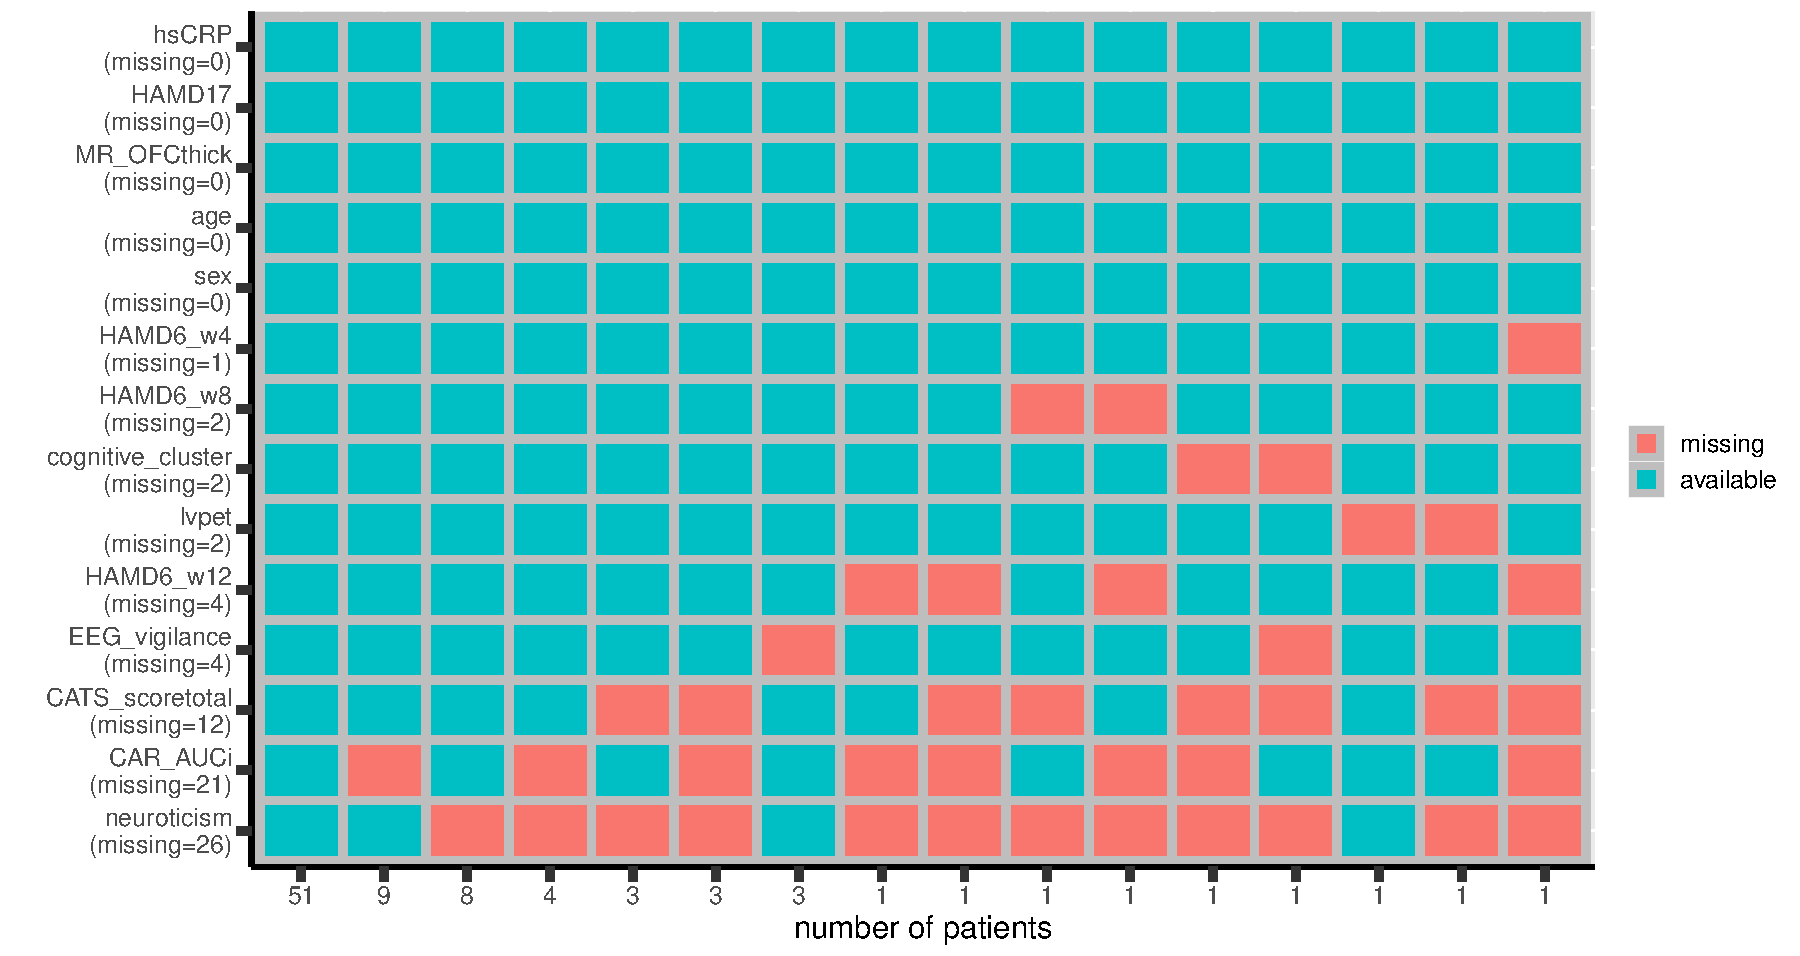
\includegraphics[trim={0 0 0 0},width=0.9\textwidth]{./figures/gg-missingPattern.pdf}
\caption{\label{fig:missingPattern}Missing data patterns}
\end{figure}


\subsection{Association study (week 8)}
\label{sec:orga1dfee0}

\textbf{Complete case}: excluding CATS, CAR, and neuroticism, we fitted two
logistic regressions (one with and one without the biomarkers) on the
75 patients with complete data. This likelihood ratio test showed
evidence for an association between biomarkers and recovery:
\begin{verbatim}
Analysis of Deviance Table

Model 1: Y_w8 ~ female + age
Model 2: Y_w8 ~ female + age + MR_OFCthick + HAMD17 + low_hsCRP + lvpet + 
    cognitive_cluster2 + cognitive_cluster3 + EEG_vigilance
  Resid. Df Resid. Dev Df Deviance Pr(>Chi)   
1        72    100.696                        
2        65     80.818  7   19.878  0.00584 **
---
Signif. codes:  0 '***' 0.001 '**' 0.01 '*' 0.05 '.' 0.1 ' ' 1
\end{verbatim}

Looking at the biomarker specific effects, high vigilance appeared to
be associated with poor recovery: odd ratio 0.179 (unit?) adjusted
p-value of 0.047. There was also a similar trend for cognitive cluster
3: odd ratio 0.15, adjusted p-value of 0.07.
\begin{verbatim}
                      estimate  std.error    odd ratio     p.value adjusted p-value
(Intercept)         9.15328187 8.39872601 9.445388e+03 0.275782879               NA
female             -0.35932885 0.64097717 6.981447e-01 0.575073390               NA
age                 0.05471804 0.04216889 1.056243e+00 0.194427297               NA
MR_OFCthick        -5.84569691 3.18471343 2.892318e-03 0.066424416       0.23752311
HAMD17              0.16179531 0.09514669 1.175620e+00 0.089040138       0.24208663
low_hsCRP           1.46954263 0.72733733 4.347246e+00 0.043337596       0.19466776
lvpet              -2.04888723 2.23330861 1.288782e-01 0.358921367       0.41535424
cognitive_cluster2 -0.81977323 0.69278301 4.405315e-01 0.236688505       0.41535424
cognitive_cluster3 -1.89634154 0.75932143 1.501168e-01 0.012510207       0.06993304
EEG_vigilance      -1.72062639 0.63876369 1.789540e-01 0.007066751       0.04675833
\end{verbatim}

\textbf{Multiple imputation}: as a sensitivity analysis, we now used all
patients and all biomarkers and use multiple imputations (100
datasets) to handle missing value. Results are rather similar to the
complete case analysis, with a slight tendency for stronger effects.
\lstset{language=r,label= ,caption= ,captionpos=b,numbers=none}
\begin{lstlisting}
summary(pool(e.glm_impw8))[,c(1,2,3,5:6)]
\end{lstlisting}

\begin{verbatim}
                 term      estimate    std.error       df     p.value
1         (Intercept)  4.1516290163 8.6252902526 68.91234 0.631805406
2           sexfemale -0.5825951700 0.6420666199 68.66383 0.367382059
3                 age  0.0754554026 0.0456848728 68.79669 0.103163672
4         MR_OFCthick -5.9114103612 3.0378756765 68.80810 0.055751906
5              HAMD17  0.1808561403 0.0925544076 68.24495 0.054794466
6            hsCRPlow  1.6868813295 0.7699177493 67.17518 0.031925680
7               lvpet -2.6139562643 2.3770155497 68.85573 0.275301586
8  cognitive_cluster2 -1.1511850446 0.7226909239 68.23190 0.115801761
9  cognitive_cluster3 -2.7674590923 0.8726252184 68.19986 0.002273849
10      EEG_vigilance -1.9950780957 0.6945417890 68.76199 0.005411043
11    CATS_scoretotal -0.0001481392 0.0153985265 68.98892 0.992351959
12           CAR_AUCi  0.0007498367 0.0009340191 66.90661 0.424929161
13        neuroticism  0.0351547075 0.0211703226 68.99083 0.101339384
\end{verbatim}

\bigskip

\subsection{Association study (week 12)}
\label{sec:org4429a7f}

\textbf{Complete case}: excluding CATS, CAR, and neuroticism, we fitted two
logistic regressions (one with and one without the biomarkers) on the
72 patients with complete data. This likelihood ratio test showed no
clear evidence for an association between biomarkers and recovery:
\begin{verbatim}
Analysis of Deviance Table

Model 1: Y_w12 ~ female + age
Model 2: Y_w12 ~ female + age + MR_OFCthick + HAMD17 + low_hsCRP + lvpet + 
    cognitive_cluster2 + cognitive_cluster3 + EEG_vigilance
  Resid. Df Resid. Dev Df Deviance Pr(>Chi)
1        69     76.256                     
2        62     64.376  7    11.88   0.1046
\end{verbatim}


This was confirmed when looking at the biomarker specific effects. We
can also see that the biomarkers for which with have most evidence
against the null (\texttt{MR\_OFCthick} and \texttt{cognitive\_cluster2}) differ from
week 8
\begin{verbatim}
                     estimate  std.error    odd ratio    p.value adjusted p-value
(Intercept)        15.1377108 9.66268612 3.751667e+06 0.11720467               NA
female             -0.1631019 0.71162765 8.495046e-01 0.81871691               NA
age                 0.1239538 0.07958311 1.131964e+00 0.11934255               NA
MR_OFCthick        -8.2502682 3.58368566 2.611885e-04 0.02132536        0.1342289
HAMD17              0.1706117 0.10751351 1.186030e+00 0.11253840        0.4384615
low_hsCRP           1.0809026 0.83834457 2.947339e+00 0.19728347        0.5786588
lvpet              -0.5703845 2.60457709 5.653080e-01 0.82665539        0.9698902
cognitive_cluster2 -1.4448166 0.79614533 2.357893e-01 0.06956004        0.3344590
cognitive_cluster3 -0.8051151 0.88884433 4.470365e-01 0.36504179        0.7385351
EEG_vigilance      -0.0668419 0.60067967 9.353431e-01 0.91139660        0.9698902
\end{verbatim}

\textbf{Multiple imputation}: as a sensitivity analysis, we now used all
patients and all biomarkers and use multiple imputations (100
datasets) to handle missing value. Results are rather similar to the
complete case analysis, but with a stronger evidence for an assocation
between OFC thickness and recovery. Note that cognition and CATS are
bordeline significant without adjustment for multiple comparisons.
\lstset{language=r,label= ,caption= ,captionpos=b,numbers=none}
\begin{lstlisting}
summary(pool(e.glm_impw12))[,c(1,2,3,5:6)]
\end{lstlisting}

\begin{verbatim}
                 term     estimate   std.error       df     p.value
1         (Intercept) 16.760516575 9.890355948 65.99623 0.094859430
2           sexfemale -0.898638556 0.731432568 65.79797 0.223597826
3                 age  0.115967103 0.075427653 66.00500 0.128960677
4         MR_OFCthick -9.520173723 3.499858676 65.92820 0.008334242
5              HAMD17  0.141151055 0.103171990 65.81972 0.175928909
6            hsCRPlow  1.004339184 0.857512761 65.03615 0.245782198
7               lvpet -0.643880653 2.660297543 65.99493 0.809504882
8  cognitive_cluster2 -1.906920071 0.887507143 65.52557 0.035364314
9  cognitive_cluster3 -1.725228423 0.949783976 65.71480 0.073863526
10      EEG_vigilance -0.382219479 0.630217817 66.01354 0.546270922
11    CATS_scoretotal  0.037284123 0.020188426 66.02463 0.069257123
12           CAR_AUCi  0.001358667 0.001228576 65.78712 0.272803070
13        neuroticism  0.017883788 0.023653524 65.95409 0.452297597
\end{verbatim}

\subsection{Predictive value (week 8)}
\label{sec:org68ddcb4}

\textbf{Complete case}: excluding CATS, CAR, and neuroticism, we assessed the
predictive performance of two logistic regressions (one with
\texttt{glm\_ccw8} and one without the biomarkers \texttt{glm0\_ccw8}) as well as a
random forest model (\texttt{rf\_ccw8}) on the 75 patients with complete data:
\begin{verbatim}
     method metric     model   estimate
1  internal    auc glm0_ccw8 0.62769010
2  internal    auc  glm_ccw8 0.81133429
3  internal    auc   rf_ccw8 1.00000000
4  internal  brier glm0_ccw8 0.23870239
5  internal  brier  glm_ccw8 0.17485453
6  internal  brier   rf_ccw8 0.09276568
7        cv    auc glm0_ccw8 0.52305595
8        cv    auc  glm_ccw8 0.67530846
9        cv    auc   rf_ccw8 0.55341822
10       cv  brier glm0_ccw8 0.25887838
11       cv  brier  glm_ccw8 0.23932881
12       cv  brier   rf_ccw8 0.25372824
\end{verbatim}

After cross-validation, we observe that both the AUC and brier score
of the random forest (with biomarkers) are similar to the logistic
regression without biomarkers. This indicates poor predictive ability
of the random forest that will not be considered further. The logistic
model with biomarker has a higher AUC (i.e., better discrimination)
and lower brier score (i.e., smaller discrepancy between prediction
and observed outcome) compared to the logistic model without
biomarkers. The permutation test confirmed that the logistic model
with biomarkers was informative (p=0.02 for the AUC and p=0.01 for the
brier score \Warning \textcolor{red}{to re-run with more
permutations}) while there was no clear evidence with the logistic
model without covariates (p=0.11 for the AUC and p=0.27 for the brier
score). This difference between the predictions from the models (after
cross validation) is illustrated in \autoref{fig:predW8}, as well as
the corresponding ROC \autoref{fig:rocW8} and calibration curves
\autoref{fig:caliW8}.

\bigskip

Note that the average AUC estimated by the permutation test was 0.5,
supporting that the proposed cross-validation procedure is unbiased
(under the null).

\clearpage

\begin{figure}[!h]
\centering
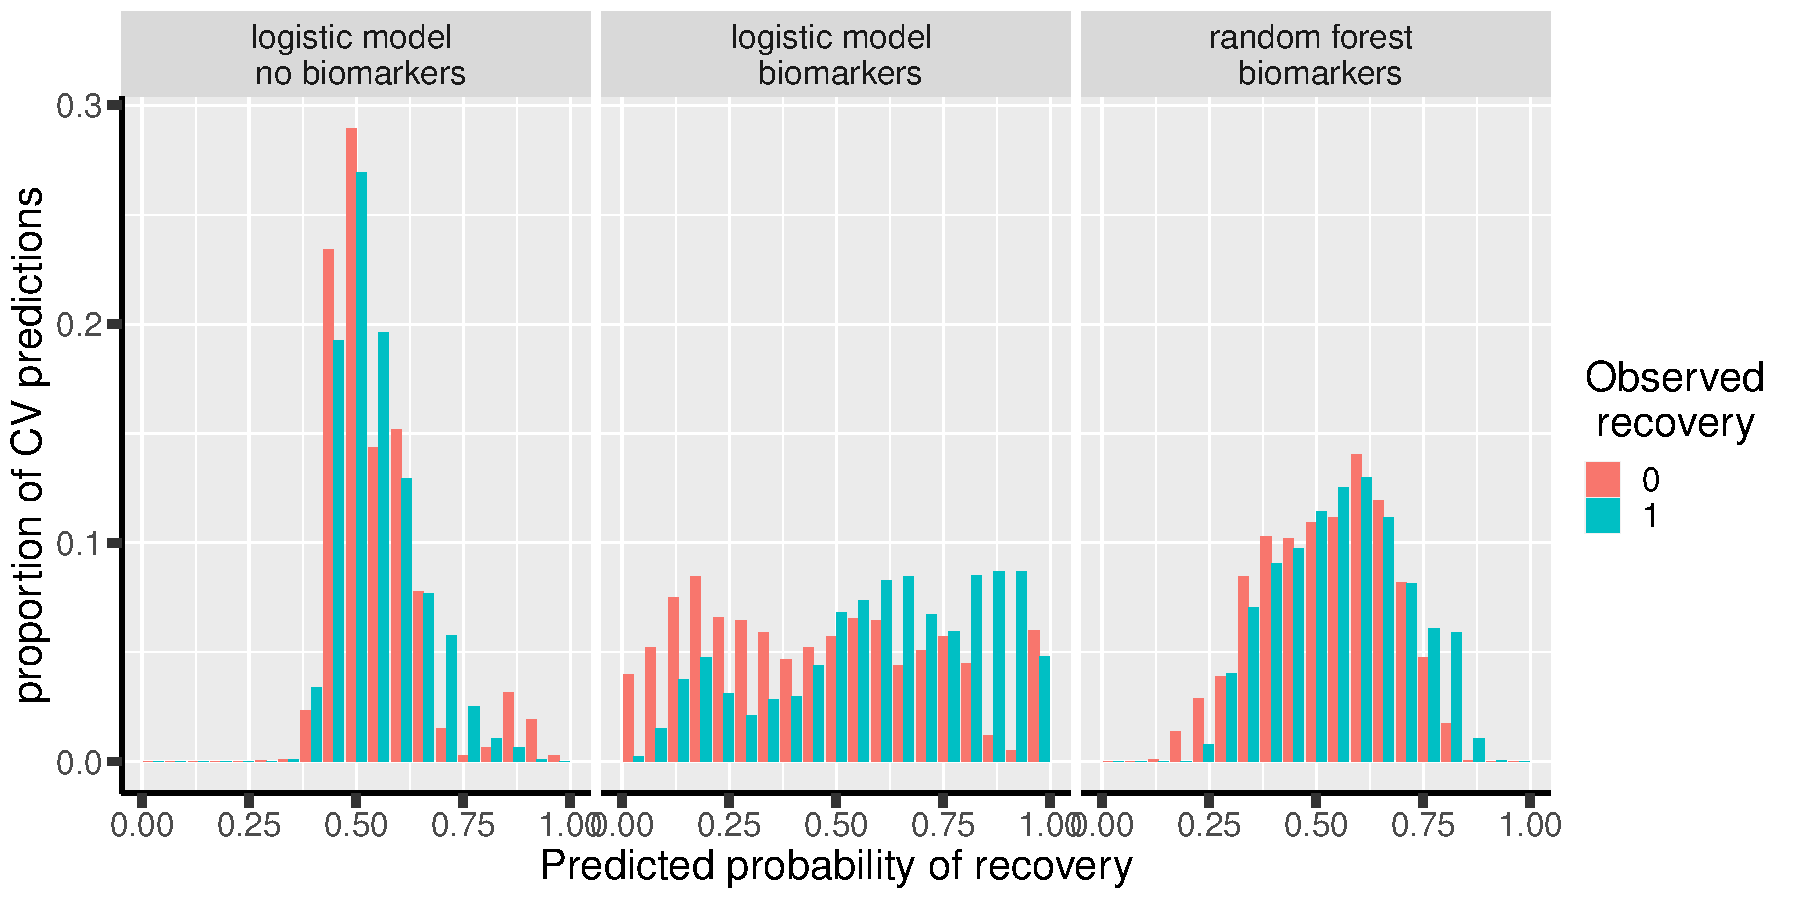
\includegraphics[trim={0 0 0 0},width=1\textwidth]{./figures/gg-perfW8-hist2.pdf}
\caption{\label{fig:predW8}Distribution of the predicted probability of recovery according to the actual recovery for the various predictive models for week 8.}
\end{figure}

\begin{figure}[!h]
\centering
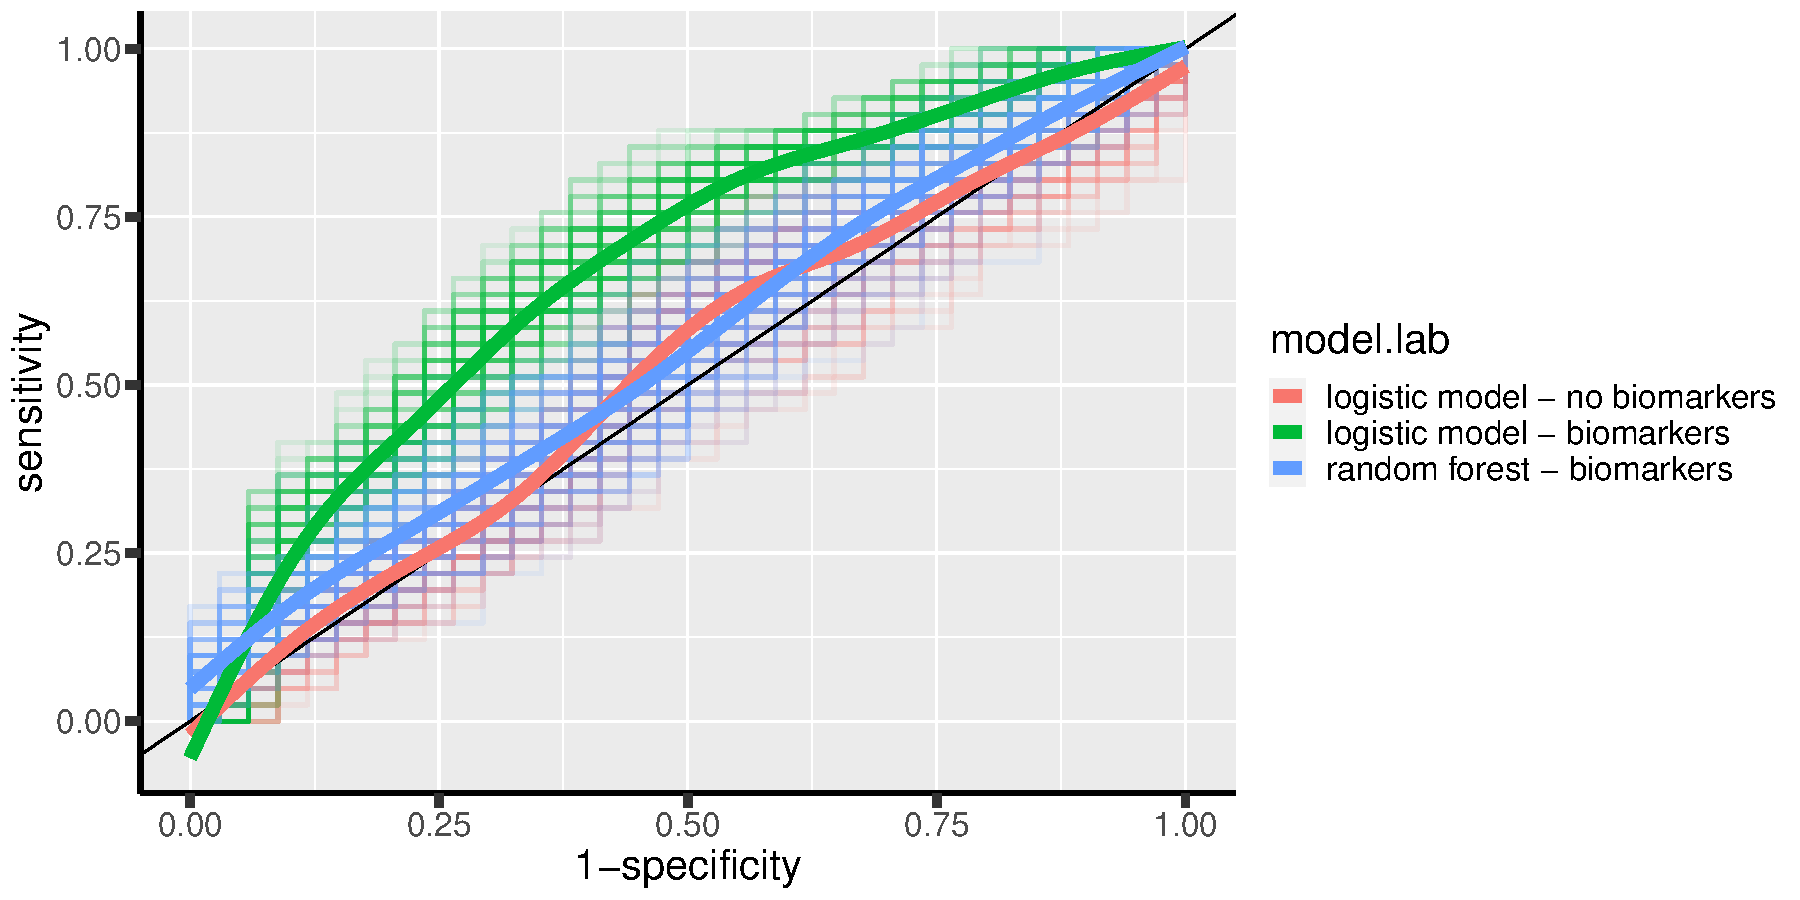
\includegraphics[trim={0 0 0 0},width=1\textwidth]{./figures/gg-perfW8-roc.pdf}
\caption{\label{fig:rocW8}Roc curve associated to the cross-validated predictions for the various models (thick lines) for week 8. It is obtained by applying a smoother (lowess) on the 100 ROC curve obtain for each model and each of the 100 repetitions of the 10 fold cross validations (thin lines).}
\end{figure}

\clearpage

\begin{figure}[!h]
\centering
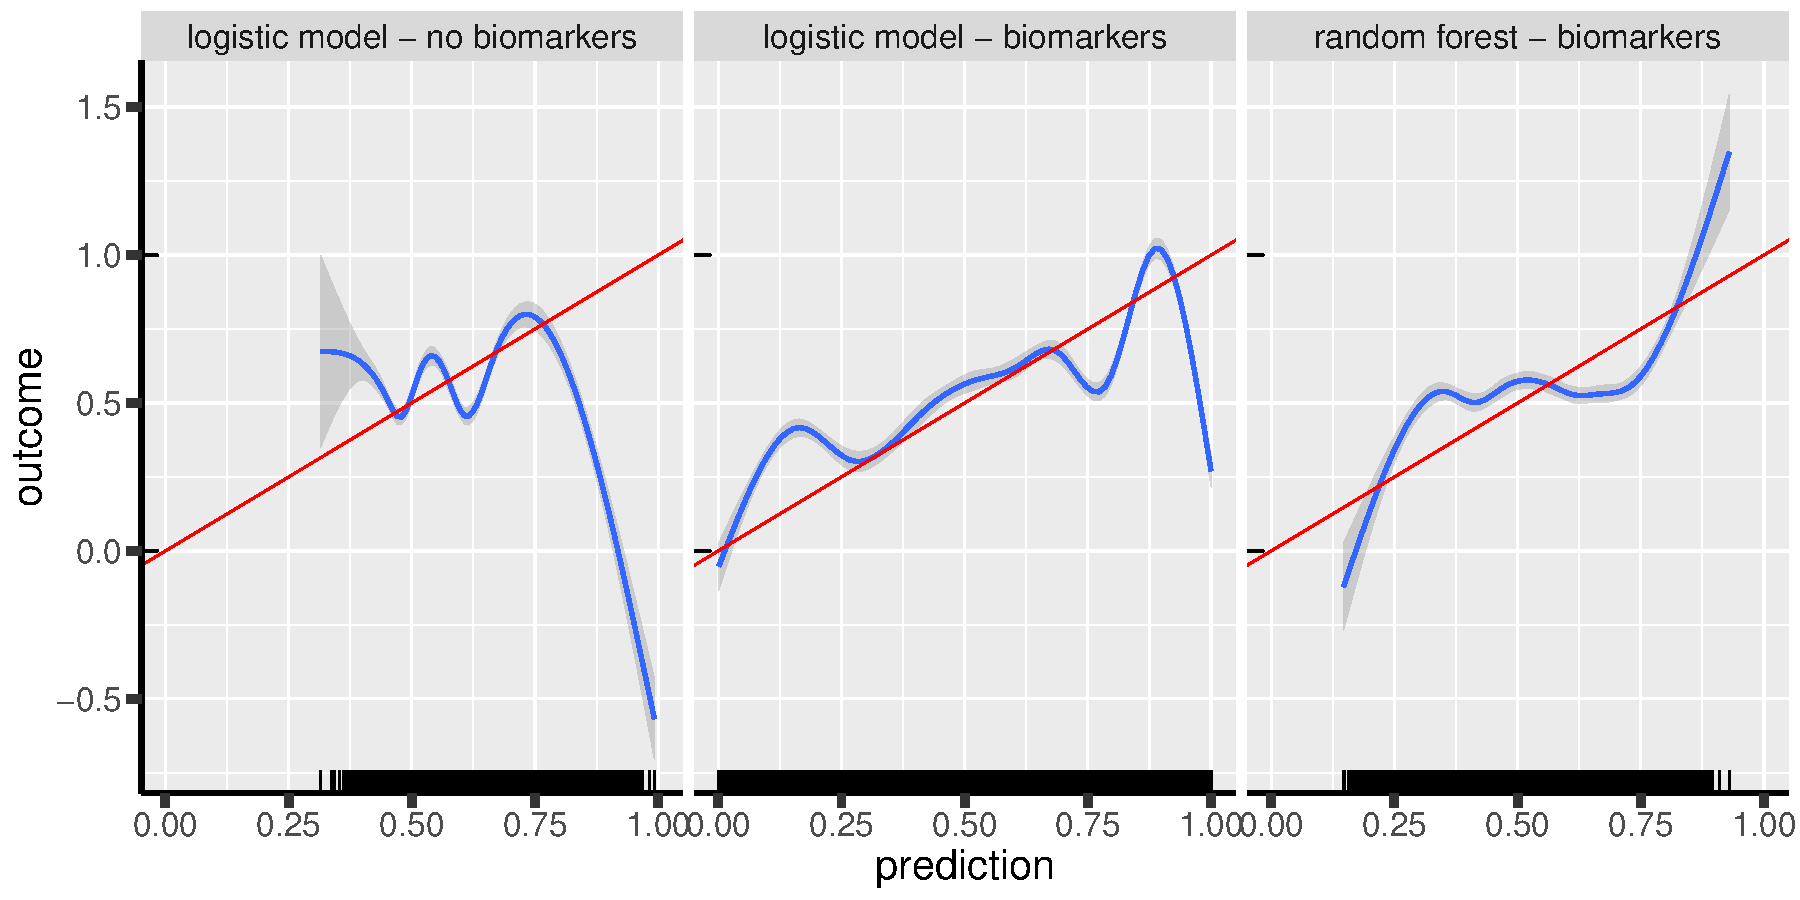
\includegraphics[trim={0 0 0 0},width=1\textwidth]{./figures/gg-perfW8-cali.pdf}
\caption{\label{fig:caliW8}Calibration curve associated to the cross-validated predictions for the various models (thick lines) for week 8.}
\end{figure}

\bigskip

\textbf{Full data}: as a sensitivity analysis, we now used all patients and
all biomarkers and modified the cross-validation procedure to handle
missing data. We obtain slightly different results, but still in favor
of the logistic model with biomarkers. The difference in AUC between
the logistic models is similar to previously (about +0.1) but now the
brier score is worse (+0.4 instead of 0.3) indicating poor
calibration.

\begin{verbatim}
     method metric   model  estimate
1: internal    auc glm0_w8 0.5991949
2: internal    auc  glm_w8 0.8878666
3: internal  brier glm0_w8 0.2409137
4: internal  brier  glm_w8 0.1432597
5:       cv    auc glm0_w8 0.5574226
6:       cv    auc  glm_w8 0.6542563
7:       cv  brier glm0_w8 0.2581057
8:       cv  brier  glm_w8 0.3015577
\end{verbatim}



\clearpage

\subsection{Predictive value (week 12)}
\label{sec:org0464d4e}

\textbf{Complete case}: excluding CATS, CAR, and neuroticism, we assessed the
predictive performance of two logistic regressions (one with
\texttt{glm\_ccw12} and one without the biomarkers \texttt{glm0\_ccw12}) as well as a
random forest model (\texttt{rf\_ccw12}) on the 72 patients with complete data:
\begin{verbatim}
     method metric      model   estimate
1  internal    auc glm0_ccw12 0.66037736
2  internal    auc  glm_ccw12 0.79443893
3  internal    auc   rf_ccw12 1.00000000
4  internal  brier glm0_ccw12 0.18160078
5  internal  brier  glm_ccw12 0.14937617
6  internal  brier   rf_ccw12 0.05981177
7        cv    auc glm0_ccw12 0.57554121
8        cv    auc  glm_ccw12 0.60582920
9        cv    auc   rf_ccw12 0.76768620
10       cv  brier glm0_ccw12 0.19544784
11       cv  brier  glm_ccw12 0.21388319
12       cv  brier   rf_ccw12 0.16378866
\end{verbatim}

After cross-validation, we observe that both the AUC and brier score
of the logistic regression with biomarkers are similar to the logistic
regression without biomarkers. This time it the random forest approach
that shows a higher AUC (i.e., better discrimination) and lower brier
score (i.e., smaller discrepancy between prediction and observed
outcome) compared to the logistic model without biomarkers. The
permutation test confirmed that the logistic model with biomarkers was
informative (p=0.01 for the AUC and p=0.01 for the brier score
\Warning \textcolor{red}{to re-run with more permutations}) while
there was no clear evidence for the other logistic models (p>0.1 for
the AUC and brier score). This difference between the predictions from
the models (after cross validation) is illustrated in
\autoref{fig:predW12}, as well as the corresponding ROC
\autoref{fig:rocW12} and calibration curves \autoref{fig:caliW12}.

\bigskip

Note that the average AUC estimated by the permutation test was 0.5,
supporting that the proposed cross-validation procedure is unbiased
(under the null).

\clearpage

\begin{figure}[!h]
\centering
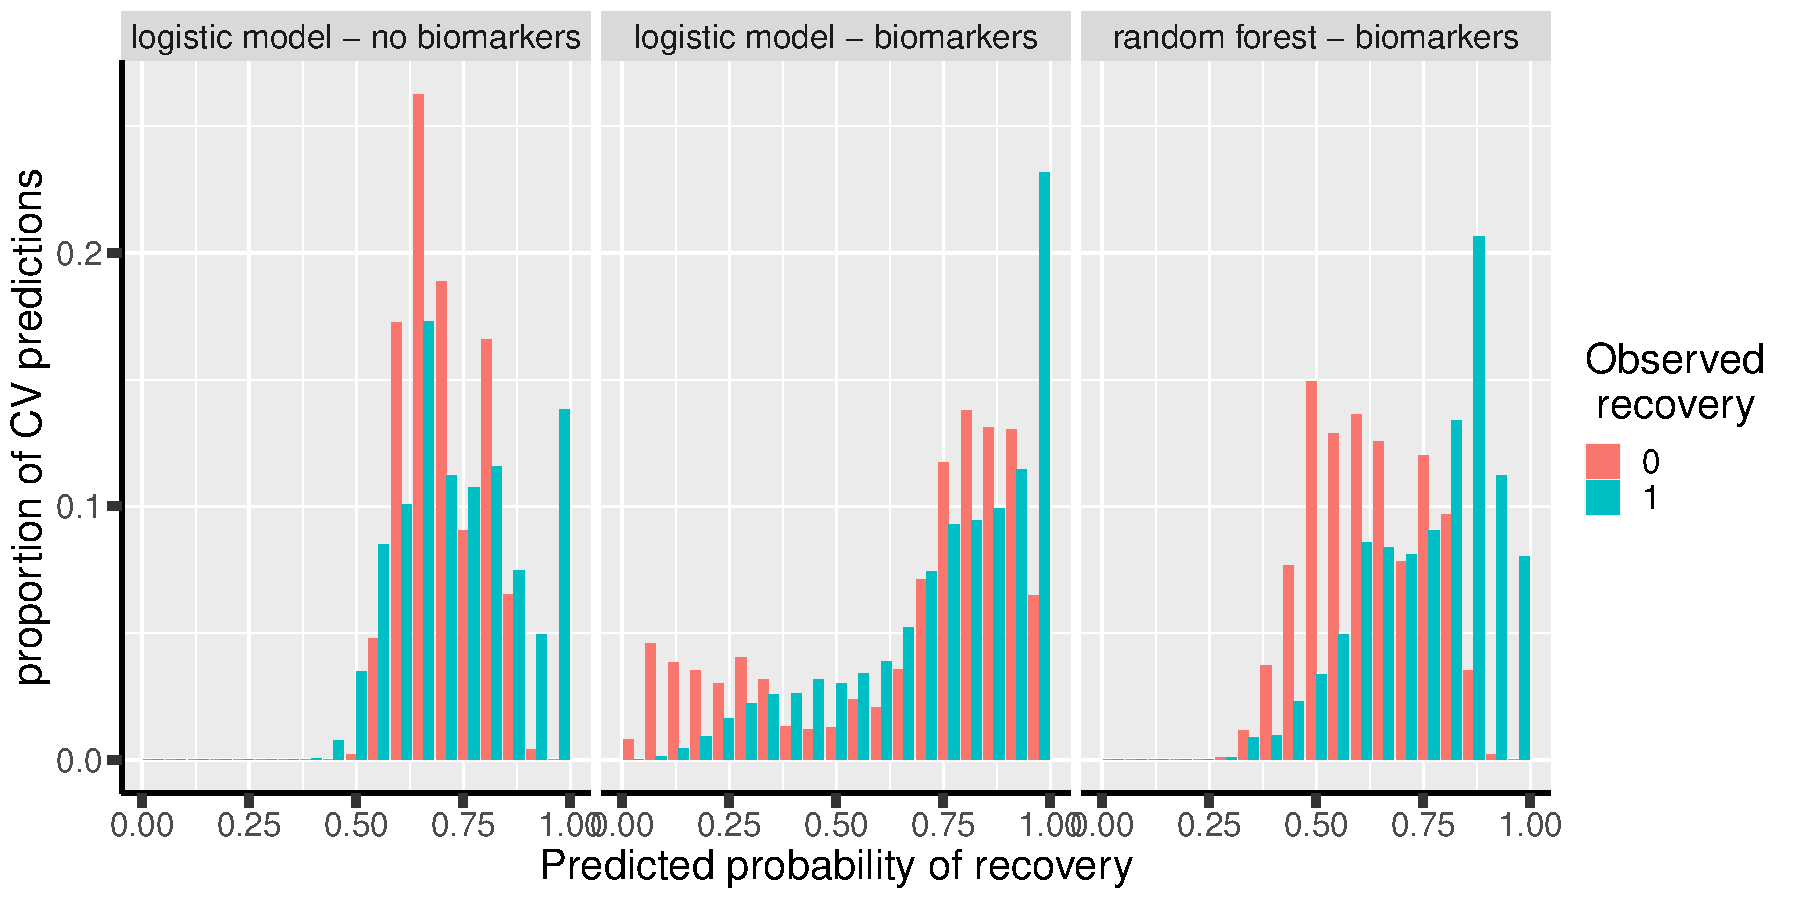
\includegraphics[trim={0 0 0 0},width=1\textwidth]{./figures/gg-perfW12-hist2.pdf}
\caption{\label{fig:predW12}Distribution of the predicted probability of recovery according to the actual recovery for the various predictive models for week 12.}
\end{figure}

\begin{figure}[!h]
\centering
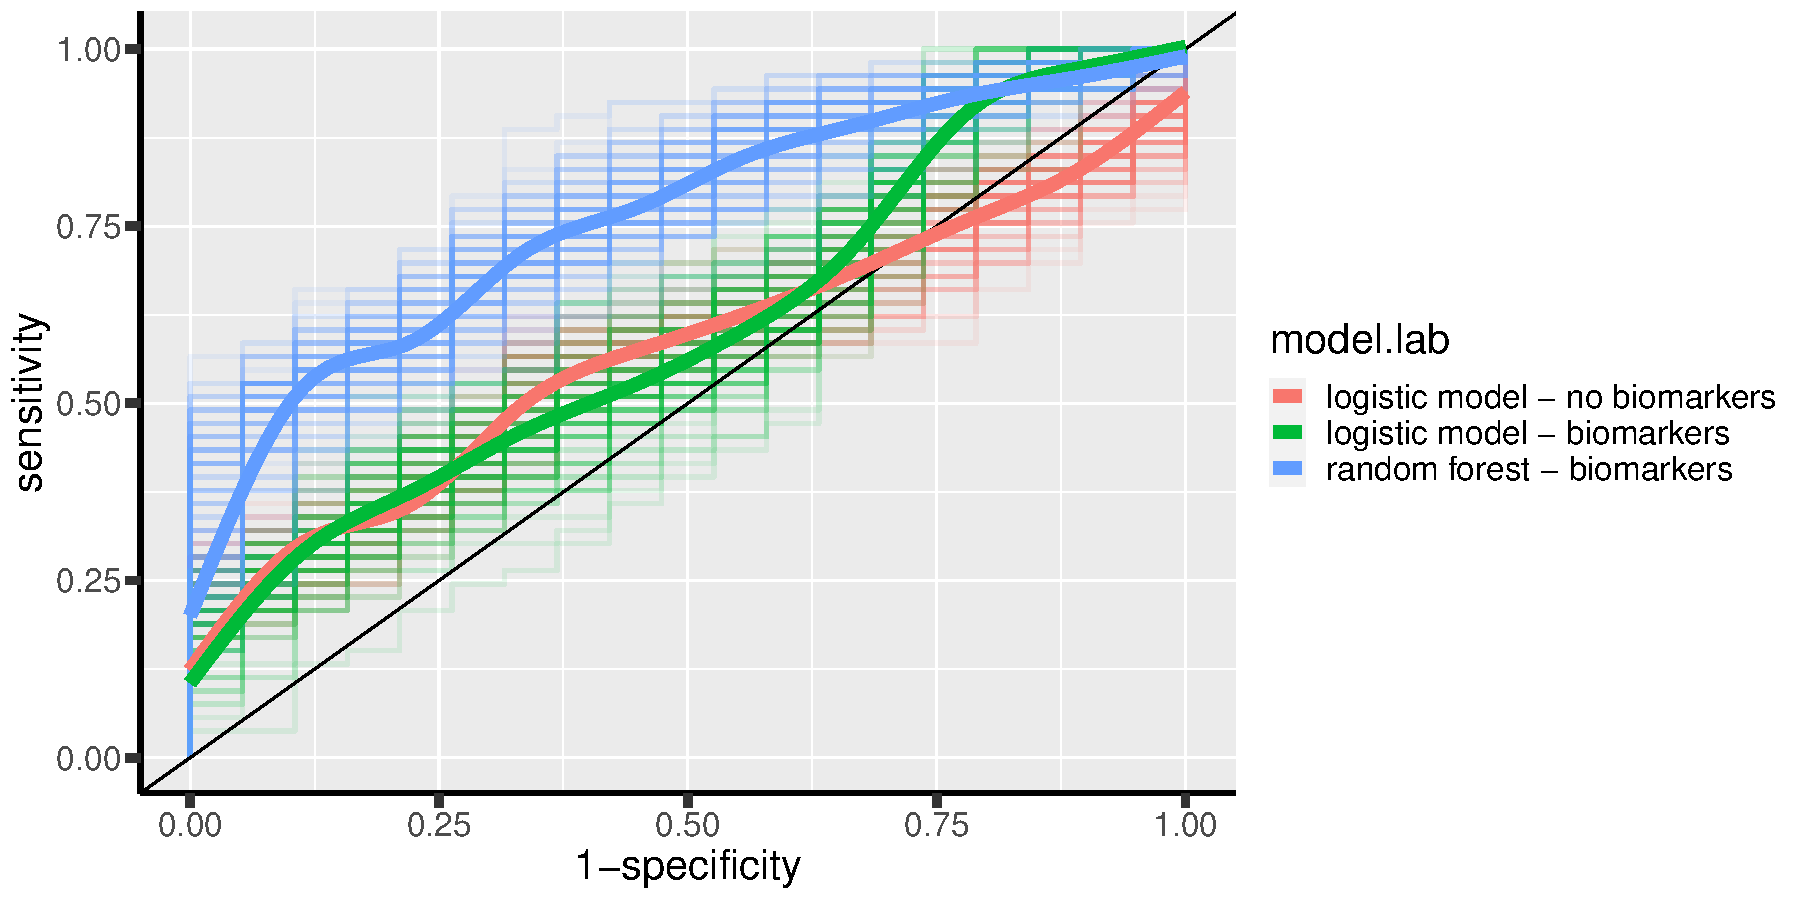
\includegraphics[trim={0 0 0 0},width=1\textwidth]{./figures/gg-perfW12-roc.pdf}
\caption{\label{fig:rocW12}Roc curve associated to the cross-validated predictions for the various models (thick lines) for week 12. It is obtained by applying a smoother (lowess) on the 100 ROC curve obtain for each model and each of the 100 repetitions of the 10 fold cross validations (thin lines).}
\end{figure}


\clearpage

\begin{figure}[!h]
\centering
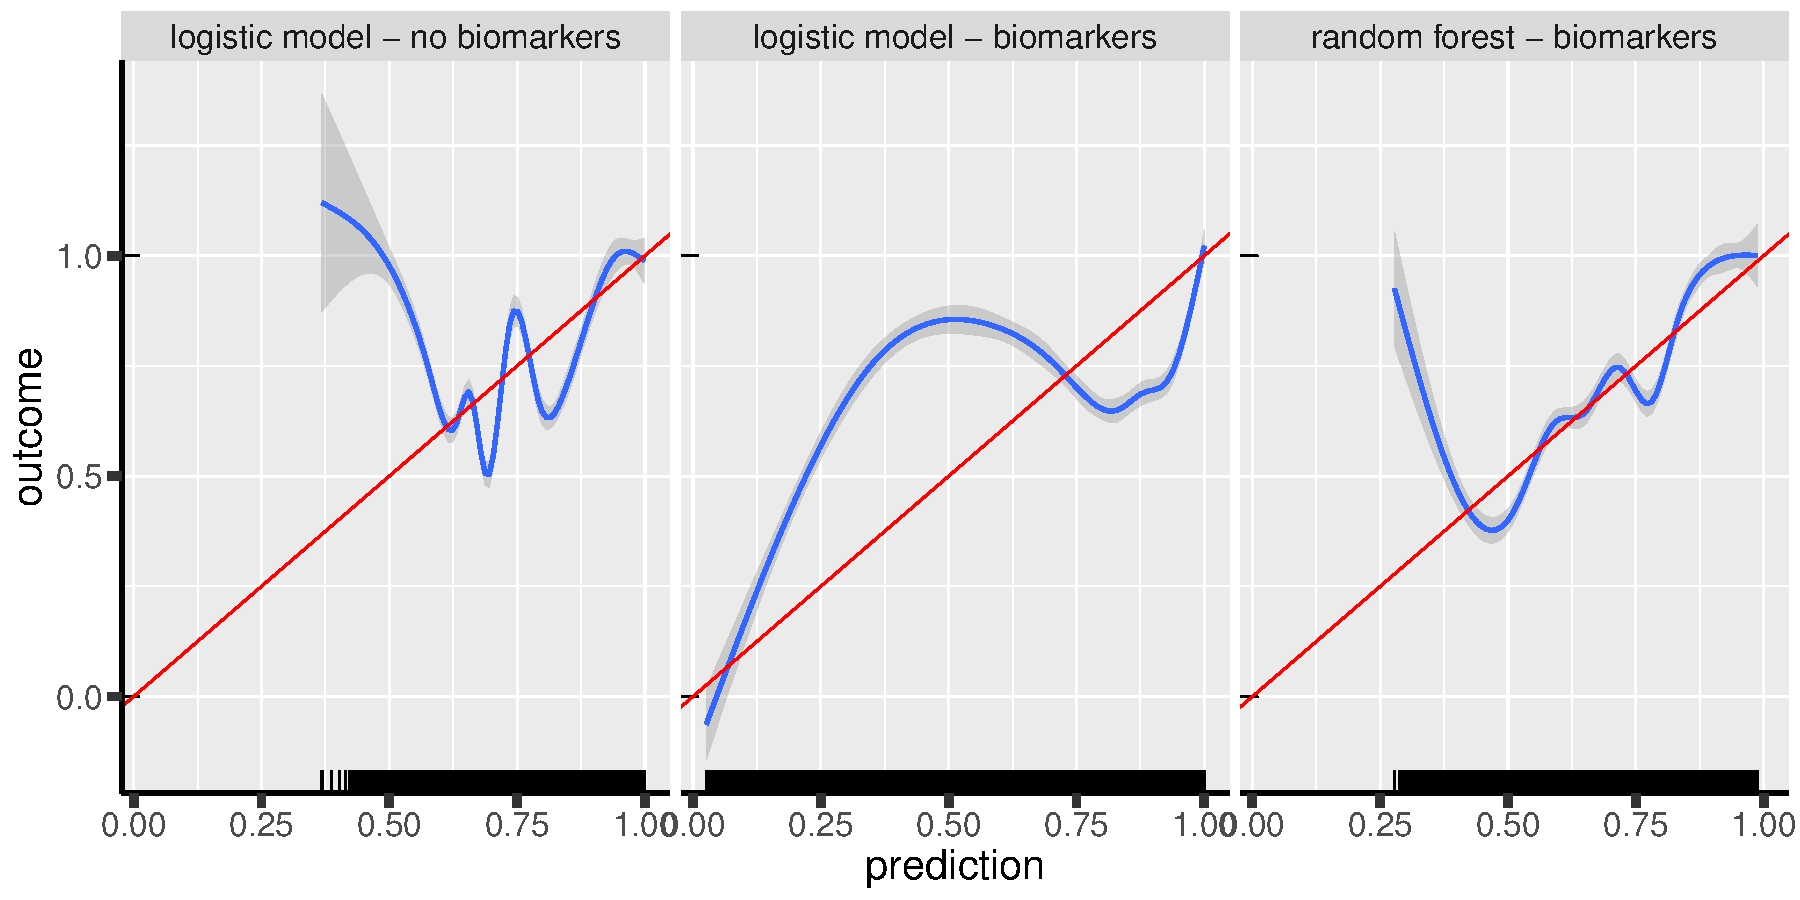
\includegraphics[trim={0 0 0 0},width=1\textwidth]{./figures/gg-perfW12-cali.pdf}
\caption{\label{fig:caliW12}Calibration curve associated to the cross-validated predictions for the various models (thick lines) for week 12.}
\end{figure}


\textbf{Full data}: as a sensitivity analysis, we now used all patients and
all biomarkers and modified the cross-validation procedure to handle
missing data. The results are in line with the complete case, with
worse performances when adding the biomarkers.

\begin{verbatim}
     method metric    model  estimate
1: internal    auc glm0_w12 0.6502311
2: internal    auc  glm_w12 0.8936826
3: internal  brier glm0_w12 0.1855812
4: internal  brier  glm_w12 0.1172801
5:       cv    auc glm0_w12 0.6017917
6:       cv    auc  glm_w12 0.5762885
7:       cv  brier glm0_w12 0.2181458
8:       cv  brier  glm_w12 0.2679212
\end{verbatim}


\clearpage

\section{Conclusion}
\label{sec:orgcd6bdc4}

There is evidence that some biomarkers (EEG, to a lesser extend
cognition) are predictive of recovery at week 8. The corresponding
gain in AUC was about +0.1 with a small improvement in brier
score. These results were not seen at week 12 and the overall
predictive performance was not great though (AUC of about 0.6 and
brier score >0.2).

\bigskip

There was no evidence for non-linear effect or interaction between
biomarkers (as assessed via a random forest model) probably due to the
limited sample size.

\bigskip

Generally the results where robust to how missing data were handled
  (complete case or multiple imputation). Effects had a slight
  tendency to be stronger when not using complete case. The only
  exception is for the brier score at w8 which became worse compared
  to the complete case.  \bigskip


\section{References}
\label{sec:org2d2c201}
\begingroup
\renewcommand{\section}[2]{}
\bibliographystyle{apalike}
\bibliography{bibliography}

\endgroup
\end{document}